\subsubsection{Calendarización - Dar orden y tiempo al trabajo [Pendientes: 1. Elaborar la carta Gantt de 2027-1 con fechas, duraciones y dependencias, detallando las actividades repetitivas de una sola iteración, y elaborar un diagrama BPMN para representar el flujo recurrente de trabajo. 2. Acordar iteraciones, agenda, revisiones y periodos de corrección. 3. Establecer la actualización de la carta Gantt en cada entrega para reflejar el avance real del proyecto.]}\label{sec:spmp-9-3-2}

La figura presenta la calendarización propuesta para 2027-1 con base en las iteraciones de la sección~\ref{sec:spmp-8-1} y las dependencias de la sección~\ref{sec:spmp-9-3-1}. Las fechas de acceso a HPC-ZINE, evaluación con usuarios y entrega están sujetas a confirmación. La semana del 22 al 28 de marzo corresponde a trabajo individual de baja carga.

\begin{landscape}
\begin{figure}[p]\centering
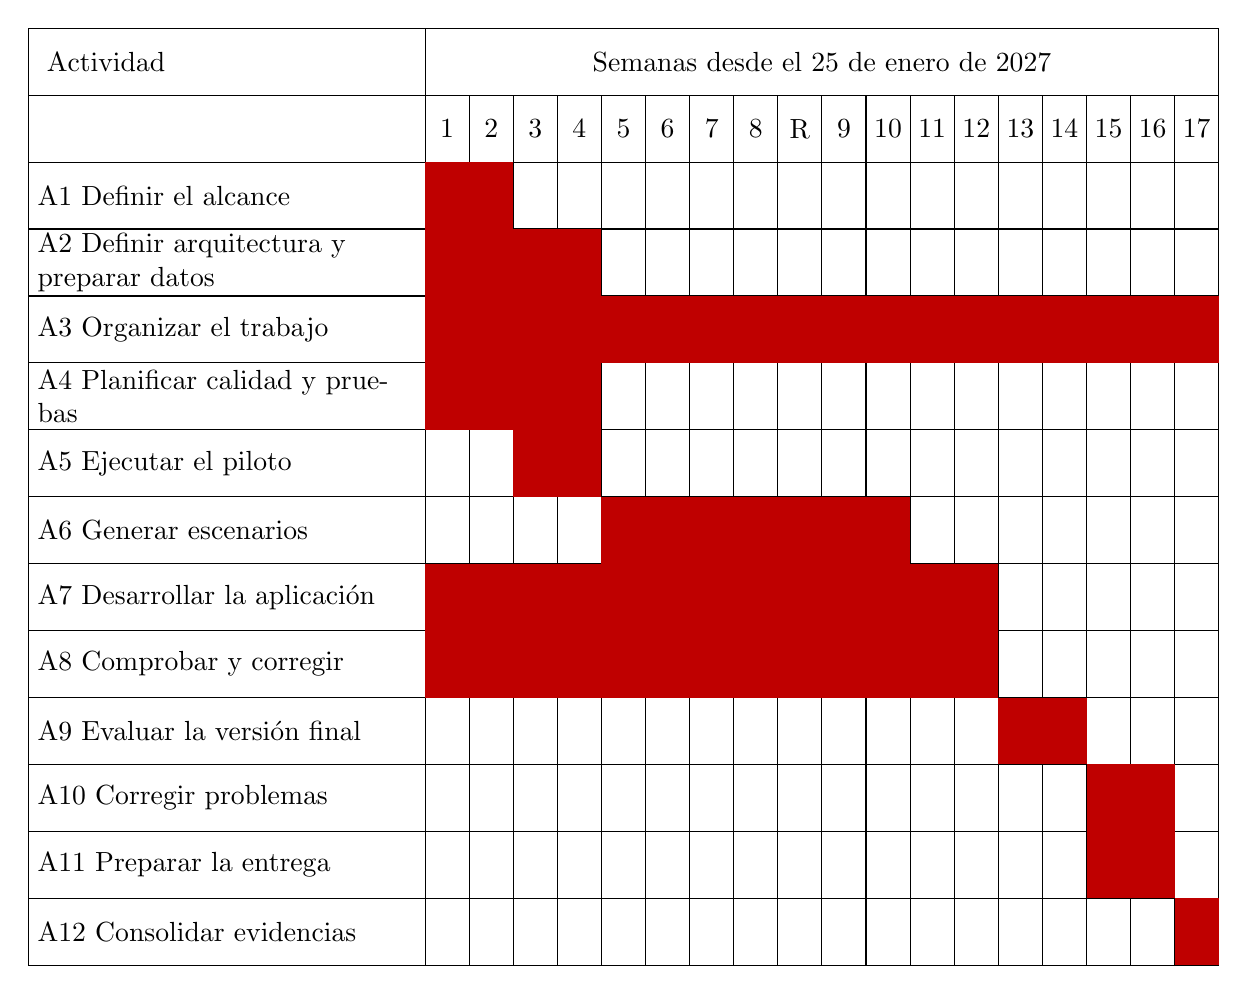
\begin{tikzpicture}[x=0.56cm,y=0.85cm,font=\normalsize]
\draw (0,0) rectangle (27,-14);
\foreach \y in {1,...,13} \draw (0,-\y)--(27,-\y);
\draw (9,0)--(9,-14);
\foreach \x in {10,...,26} \draw (\x,-1)--(\x,-14);
\node[anchor=west] at (0.2,-0.5) {Actividad};
\node at (18,-0.5) {Semanas desde el 25 de enero de 2027};
\node at (9.5,-1.5) {1};
\node at (10.5,-1.5) {2};
\node at (11.5,-1.5) {3};
\node at (12.5,-1.5) {4};
\node at (13.5,-1.5) {5};
\node at (14.5,-1.5) {6};
\node at (15.5,-1.5) {7};
\node at (16.5,-1.5) {8};
\node at (17.5,-1.5) {R};
\node at (18.5,-1.5) {9};
\node at (19.5,-1.5) {10};
\node at (20.5,-1.5) {11};
\node at (21.5,-1.5) {12};
\node at (22.5,-1.5) {13};
\node at (23.5,-1.5) {14};
\node at (24.5,-1.5) {15};
\node at (25.5,-1.5) {16};
\node at (26.5,-1.5) {17};
\fill[red!75!black] (9,-3) rectangle (11,-2);
\node[anchor=west,text width=4.7cm,align=left,inner sep=0pt] at (0.2,-2.5) {A1 Definir el alcance};
\fill[red!75!black] (9,-4) rectangle (13,-3);
\node[anchor=west,text width=4.7cm,align=left,inner sep=0pt] at (0.2,-3.5) {A2 Definir arquitectura y preparar datos};
\fill[red!75!black] (9,-5) rectangle (27,-4);
\node[anchor=west,text width=4.7cm,align=left,inner sep=0pt] at (0.2,-4.5) {A3 Organizar el trabajo};
\fill[red!75!black] (9,-6) rectangle (13,-5);
\node[anchor=west,text width=4.7cm,align=left,inner sep=0pt] at (0.2,-5.5) {A4 Planificar calidad y pruebas};
\fill[red!75!black] (11,-7) rectangle (13,-6);
\node[anchor=west,text width=4.7cm,align=left,inner sep=0pt] at (0.2,-6.5) {A5 Ejecutar el piloto};
\fill[red!75!black] (13,-8) rectangle (20,-7);
\node[anchor=west,text width=4.7cm,align=left,inner sep=0pt] at (0.2,-7.5) {A6 Generar escenarios};
\fill[red!75!black] (9,-9) rectangle (22,-8);
\node[anchor=west,text width=4.7cm,align=left,inner sep=0pt] at (0.2,-8.5) {A7 Desarrollar la aplicación};
\fill[red!75!black] (9,-10) rectangle (22,-9);
\node[anchor=west,text width=4.7cm,align=left,inner sep=0pt] at (0.2,-9.5) {A8 Comprobar y corregir};
\fill[red!75!black] (22,-11) rectangle (24,-10);
\node[anchor=west,text width=4.7cm,align=left,inner sep=0pt] at (0.2,-10.5) {A9 Evaluar la versión final};
\fill[red!75!black] (24,-12) rectangle (26,-11);
\node[anchor=west,text width=4.7cm,align=left,inner sep=0pt] at (0.2,-11.5) {A10 Corregir problemas};
\fill[red!75!black] (24,-13) rectangle (26,-12);
\node[anchor=west,text width=4.7cm,align=left,inner sep=0pt] at (0.2,-12.5) {A11 Preparar la entrega};
\fill[red!75!black] (26,-14) rectangle (27,-13);
\node[anchor=west,text width=4.7cm,align=left,inner sep=0pt] at (0.2,-13.5) {A12 Consolidar evidencias};
\end{tikzpicture}
\caption{Carta Gantt semanal propuesta para 2027-1. Fuente: elaboración propia.}\label{fig:gantt-proyecto}
\end{figure}
\end{landscape}

Las semanas 1 a 17 corresponden al calendario académico. La columna R representa el receso de Semana Santa, del 22 al 28 de marzo, con trabajo individual de baja carga; no se cuenta como semana de trabajo. La semana 17 comprende del 24 al 29 de mayo y se destina a la entrega final. Las versiones iniciales de A1 a A4 se preparan en Inicio; las barras muestran su refinamiento y seguimiento en 2027-1. La preparación de datos y el acceso a HPC preceden al piloto A5; su comprobación precede a A6. A7 y sus pruebas A8 avanzan en paralelo con A6; la integración de la aplicación con la biblioteca estable precede a la evaluación A9. Esta precede a las correcciones A10 y a la preparación final A11; A12 consolida las evidencias antes de la entrega.

La Figura~\ref{fig:bpmn-iteracion-ix} complementa la calendarización mediante un diagrama BPMN del flujo recurrente de una iteración genérica, mostrando la secuencia base de planificación, ejecución, verificación, integración, revisión y cierre, así como la interacción con la dirección del proyecto.

\begin{landscape}
\begin{figure}[p]
\centering
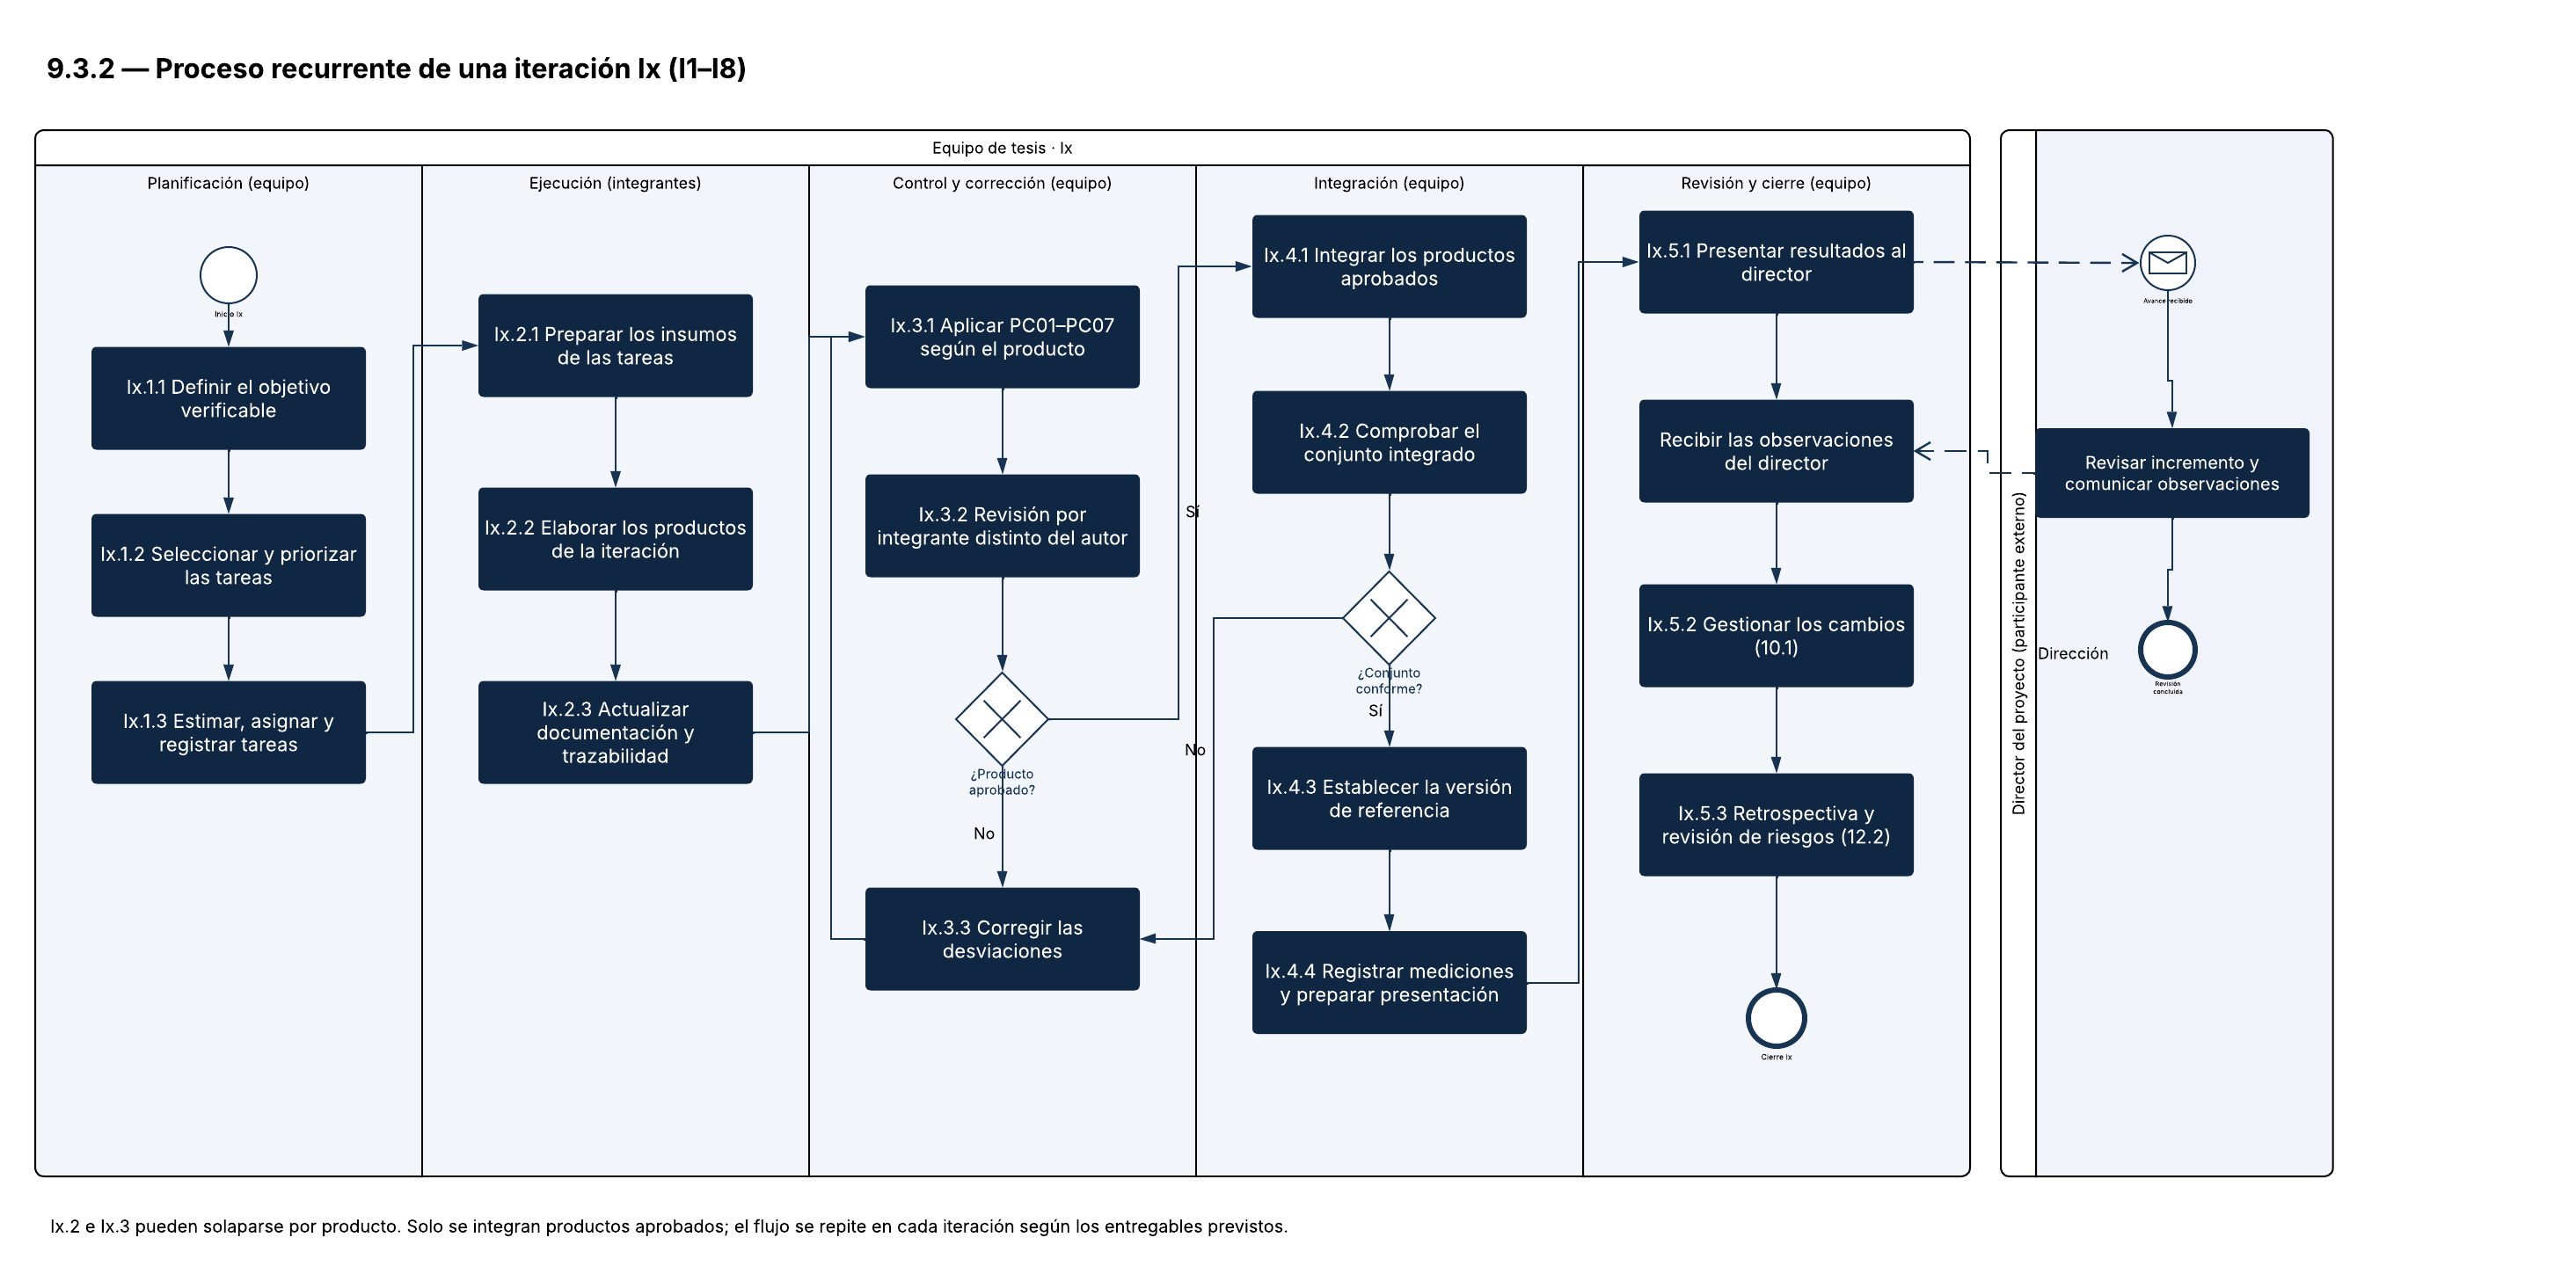
\includegraphics[width=\linewidth,height=0.82\textheight,keepaspectratio]{BPMN 9.3.2.png}
\caption{Diagrama BPMN del proceso recurrente de una iteración Ix (I1--I18). Fuente: elaboración propia.}
\label{fig:bpmn-iteracion-ix}
\end{figure}
\end{landscape}

En cada iteración se planifica el lunes de la primera semana; el jueves de la segunda se integran los cambios y se preparan mediciones y demostración; el viernes se revisan los resultados con el director y se realiza la retrospectiva, conforme a la sección~\ref{sec:spmp-8-1}. El equipo revisará el cronograma en cada entrega y registrará los ajustes siguiendo la sección~\ref{sec:spmp-6-6}.